\documentclass{standalone}
\usepackage{tikz}

\begin{document}
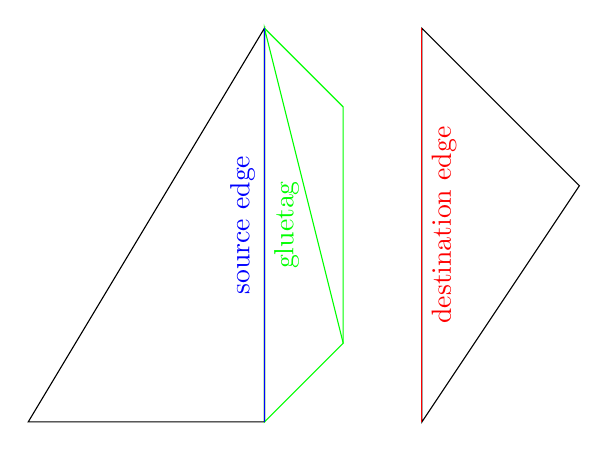
\begin{tikzpicture}

\draw (1,1) -- (4,1) -- (4, 6) -- cycle;


\draw[green] (4,1) -- (5,2) -- (4,6) -- cycle;
\draw[green] (4,6) -- (5, 5) -- (5,2);

\draw (6,1) -- (6,6) -- (8, 4) -- cycle;


\draw[red] (6,1) -- (6,6)  node [midway, below, sloped] (TextNode) {destination edge};
\draw[blue] (4,1) -- (4,6)  node [midway, above, sloped] (TextNode) {source edge} node [midway, below, sloped, text=green] (TextNode) {gluetag};

\end{tikzpicture}
\end{document}